% DO NOT COMPILE THIS FILE DIRECTLY!
% This is included by the other .tex files.

\begin{frame}[t,plain]
\titlepage
\end{frame}

\begin{frame}[t]{What is this?}
\begin{itemize}
\item Beamer is a \LaTeX{} class that allows you to create presentations
\item The project home page is http://latex-beamer.sourceforge.net/
\item Beamer contains several themes, but they are a bit ugly
  \begin{itemize}
  \item But with a lot of useful features, such as navigation bars, outlines,
        etc.
  \end{itemize}
\item Torino is a pretty theme
  \begin{itemize}
  \item With a lot of useless -- but pretty -- features
  \item But without some useful features
  \item Well suited for short talks, for longer talks you should use themes
        with navigation bars
  \end{itemize}
\item Why the name?
  \begin{itemize}
  \item Other themes are named after locations of Universities or conferences
  \item Torino (Turin) is the location of Politecnico di Torino, my university
  \end{itemize}
\end{itemize}
\end{frame}

\begin{frame}[t,fragile]{How to use the theme}
\begin{itemize}
\item Install Beamer
  \begin{itemize}
  \item Some distros have a \verb!latex-beamer! package
  \end{itemize}
\item Read the Beamer documentation
  \begin{itemize}
  \item \verb!/usr/share/doc/latex-beamer/beameruserguide.pdf.gz! if you are
        using Debian
  \item \verb!doc/beameruserguide.pdf! in the source package
  \end{itemize}
\item Install the theme
  \begin{itemize}
  \item \verb!mkdir -p ~/texmf/tex/latex/beamer!\\
  \item \verb!cp *.sty ~/texmf/tex/latex/beamer!
  \end{itemize}
\item Read the example files
  \begin{itemize}
  \item \verb!chameleon.tex!: green theme, watermark and circles for bullet
        lists
  \item \verb!nouvelle.tex!: green and red theme, watermark and squares for
        bullet lists
  \item \verb!freewilly.tex!: blue theme, a logo and squares for bullet lists
  \end{itemize}
\end{itemize}
\end{frame}

\begin{frame}[t,fragile]{Theme files}
\begin{itemize}
\item Themes are composed by sub-themes for single features
\item Inner themes define how the title page, the bullet lists, margins,
      etc. work
  \begin{itemize}
    \item \verb!beamerinnerthemefancy.sty!
  \end{itemize}
\item Outer themes define how headers and footers look like
  \begin{itemize}
    \item \verb!beamerouterthemedecolines.sty!
  \end{itemize}
\item Color themes define the colors to be used in outer and inner themes
  \begin{itemize}
    \item \verb!beamercolorthemechameleon.sty!: green footers and headers
    \item \verb!beamercolorthemenouvelle.sty!: green footers, red headers and
          and frame title
    \item \verb!beamercolorthemefreewilly.sty!: blue footers, headers and
          frame title
  \end{itemize}
\item Global themes just include inner, outer and color themes
  \begin{itemize}
    \item \verb!beamerthemeTorino.sty!
  \end{itemize}
\end{itemize}
\end{frame}

\begin{frame}[t,fragile]{Configuring the theme}
\begin{itemize}
\item Beamer themes can be configured with options between \verb![! and
      \verb!]!
  \begin{itemize}
  \item \verb!\usetheme[option1 = value, option2 = value]{Torino}!
  \end{itemize}
\item If you do not specify any option, you get
  \begin{itemize}
  \item Simple title page
  \item No watermark or logo
  \item Chameleon (green) color theme
  \item Squares for bullet lists
  \end{itemize}
\item Color themes can be changed with \verb!\usecolortheme!
  \begin{itemize}
  \item \verb!\usecolortheme{nouvelle}!: green and red
  \item \verb!\usecolortheme{freewilly}!: blue
  \end{itemize}
\item A logo, shown in the upper right corner, can be choosen with the
      \verb!\logo! command
  \begin{itemize}
  \item \verb!\logo{\includegraphics[height=50px]{logo-image}}!
  \end{itemize}
\end{itemize}
\end{frame}

\begin{frame}[t,fragile]{Alternative title page}
\begin{itemize}
\item A fancy title page can be enabled with the \verb!alternativetitlepage!
      option
\item You can put a logo in the title page, just pass the file name using the
      \verb!titlepagelogo! option
\item Remember to use a plain and top-aligned frame when using alternative title
      pages:\\
      \vskip1ex
      \verb!\begin{frame}[t,plain]!\\
      \verb!\titlepage!\\
      \verb!\end{frame}!
\end{itemize}
\end{frame}

\begin{frame}[t,fragile]{Watermark}
\begin{itemize}
\item A watermark can be shown in the bottom right corner of frames
\item Use the \verb!watermark! option to set name of the image file
\item The \verb!watermarkheight! option specifies the height of the watermark
      image
\item It's a good idea to have a big image and shrink it, so it looks good
      when the slide is full screen
\item If the image height in the slide is not the same as the original one,
      you have to use the \verb!watermarkheightmult! option
  \begin{itemize}
  \item For example, if the image is 400 pixel tall but you want it to
        occupy only 100 pixels, use
        \verb![watermarkheight=100px, watermarkheightmult=4]!
  \item It's ugly but I don't know how to fix it
  \end{itemize}
\end{itemize}
\end{frame}

\watermarkoff
\begin{frame}[t,fragile]{Disabling the watermark}
\begin{itemize}
\item You may want to disable the watermark on some frames
  \begin{itemize}
  \item For example, an image could partially cover the watermark, with ugly
        results
  \end{itemize}
\item The \verb!\watermarkoff! command can be used to disable the watermark
      in the following frames
\item The \verb!\watermarkon! command restores the watermark in the following
      frames
\item If you did not specify a watermark, nothing happens
\vskip5ex
\item \verb!\watermarkoff! was used for this frame
\end{itemize}
\end{frame}
\watermarkon

\begin{frame}[t,fragile]{Other options}
\begin{itemize}
\item The \verb!pageofpages! option defines the string between the current
      page number and the total page count
  \begin{itemize}
  \item The default is ``/''
  \item The example files set \verb!pageofpages! to ``of''
  \end{itemize}
\item The \verb!bullet! option can be used to choose the symbol used in
      bullet lists
  \begin{itemize}
  \item \verb!square!: A filled square
        ({\usebeamercolor[fg]{item}\tiny\raise0.2ex\hbox{$\blacksquare$}}) for
        first and third level items, an empty square
        ({\usebeamercolor[fg]{item}\tiny\raise0.2ex\hbox{$\square$}}) for
        second level items
  \item \verb!circle!: A filled circle ({\usebeamercolor[fg]{item}$\bullet$})
        for first and third level items, an empty circle
        ({\usebeamercolor[fg]{item}$\circ$}) for second level items
  \item The default value is \verb!square!
  \end{itemize}
\item If the \verb!titleline! option is set to \verb!true!, a horizontal line
      is drawn below the title
\end{itemize}
\end{frame}

\begin{frame}
\begin{figure}
 \centering
% \framebox[\texwidth]{
 % Created by tikzDevice version 0.6.2-92-0ad2792 on 2012-11-10 03:17:29
% !TEX encoding = UTF-8 Unicode
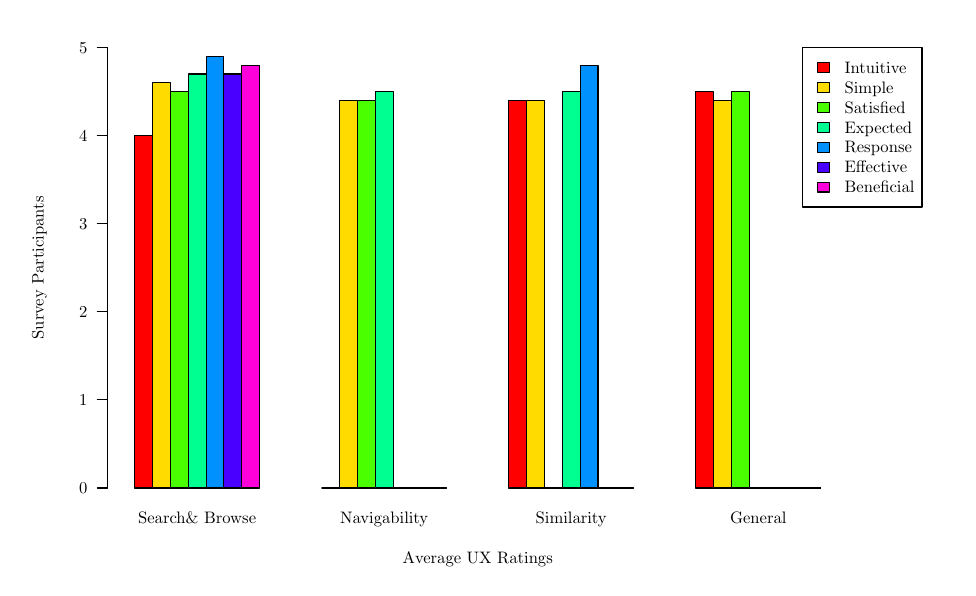
\begin{tikzpicture}[x=1pt,y=1pt]
\definecolor[named]{fillColor}{rgb}{1.00,1.00,1.00}
\path[use as bounding box,fill=fillColor,fill opacity=0.00] (0,0) rectangle (332.44,195.13);
\begin{scope}
\path[clip] (  0.00,  0.00) rectangle (332.44,195.13);
\definecolor[named]{drawColor}{rgb}{0.00,0.00,0.00}
\definecolor[named]{fillColor}{rgb}{1.00,0.00,0.00}

\path[draw=drawColor,line width= 0.4pt,line join=round,line cap=round,fill=fillColor] ( 38.71, 28.80) rectangle ( 45.15,156.10);
\definecolor[named]{fillColor}{rgb}{1.00,0.86,0.00}

\path[draw=drawColor,line width= 0.4pt,line join=round,line cap=round,fill=fillColor] ( 45.15, 28.80) rectangle ( 51.59,175.20);
\definecolor[named]{fillColor}{rgb}{0.29,1.00,0.00}

\path[draw=drawColor,line width= 0.4pt,line join=round,line cap=round,fill=fillColor] ( 51.59, 28.80) rectangle ( 58.02,172.02);
\definecolor[named]{fillColor}{rgb}{0.00,1.00,0.57}

\path[draw=drawColor,line width= 0.4pt,line join=round,line cap=round,fill=fillColor] ( 58.02, 28.80) rectangle ( 64.46,178.38);
\definecolor[named]{fillColor}{rgb}{0.00,0.57,1.00}

\path[draw=drawColor,line width= 0.4pt,line join=round,line cap=round,fill=fillColor] ( 64.46, 28.80) rectangle ( 70.90,184.75);
\definecolor[named]{fillColor}{rgb}{0.29,0.00,1.00}

\path[draw=drawColor,line width= 0.4pt,line join=round,line cap=round,fill=fillColor] ( 70.90, 28.80) rectangle ( 77.33,178.38);
\definecolor[named]{fillColor}{rgb}{1.00,0.00,0.86}

\path[draw=drawColor,line width= 0.4pt,line join=round,line cap=round,fill=fillColor] ( 77.33, 28.80) rectangle ( 83.77,181.56);
\definecolor[named]{fillColor}{rgb}{1.00,0.00,0.00}

\path[draw=drawColor,line width= 0.4pt,line join=round,line cap=round,fill=fillColor] (106.30, 28.80) rectangle (112.74, 28.80);
\definecolor[named]{fillColor}{rgb}{1.00,0.86,0.00}

\path[draw=drawColor,line width= 0.4pt,line join=round,line cap=round,fill=fillColor] (112.74, 28.80) rectangle (119.17,168.83);
\definecolor[named]{fillColor}{rgb}{0.29,1.00,0.00}

\path[draw=drawColor,line width= 0.4pt,line join=round,line cap=round,fill=fillColor] (119.17, 28.80) rectangle (125.61,168.83);
\definecolor[named]{fillColor}{rgb}{0.00,1.00,0.57}

\path[draw=drawColor,line width= 0.4pt,line join=round,line cap=round,fill=fillColor] (125.61, 28.80) rectangle (132.05,172.02);
\definecolor[named]{fillColor}{rgb}{0.00,0.57,1.00}

\path[draw=drawColor,line width= 0.4pt,line join=round,line cap=round,fill=fillColor] (132.05, 28.80) rectangle (138.48, 28.80);
\definecolor[named]{fillColor}{rgb}{0.29,0.00,1.00}

\path[draw=drawColor,line width= 0.4pt,line join=round,line cap=round,fill=fillColor] (138.48, 28.80) rectangle (144.92, 28.80);
\definecolor[named]{fillColor}{rgb}{1.00,0.00,0.86}

\path[draw=drawColor,line width= 0.4pt,line join=round,line cap=round,fill=fillColor] (144.92, 28.80) rectangle (151.36, 28.80);
\definecolor[named]{fillColor}{rgb}{1.00,0.00,0.00}

\path[draw=drawColor,line width= 0.4pt,line join=round,line cap=round,fill=fillColor] (173.89, 28.80) rectangle (180.32,168.83);
\definecolor[named]{fillColor}{rgb}{1.00,0.86,0.00}

\path[draw=drawColor,line width= 0.4pt,line join=round,line cap=round,fill=fillColor] (180.32, 28.80) rectangle (186.76,168.83);
\definecolor[named]{fillColor}{rgb}{0.29,1.00,0.00}

\path[draw=drawColor,line width= 0.4pt,line join=round,line cap=round,fill=fillColor] (186.76, 28.80) rectangle (193.20, 28.80);
\definecolor[named]{fillColor}{rgb}{0.00,1.00,0.57}

\path[draw=drawColor,line width= 0.4pt,line join=round,line cap=round,fill=fillColor] (193.20, 28.80) rectangle (199.63,172.02);
\definecolor[named]{fillColor}{rgb}{0.00,0.57,1.00}

\path[draw=drawColor,line width= 0.4pt,line join=round,line cap=round,fill=fillColor] (199.63, 28.80) rectangle (206.07,181.56);
\definecolor[named]{fillColor}{rgb}{0.29,0.00,1.00}

\path[draw=drawColor,line width= 0.4pt,line join=round,line cap=round,fill=fillColor] (206.07, 28.80) rectangle (212.51, 28.80);
\definecolor[named]{fillColor}{rgb}{1.00,0.00,0.86}

\path[draw=drawColor,line width= 0.4pt,line join=round,line cap=round,fill=fillColor] (212.51, 28.80) rectangle (218.94, 28.80);
\definecolor[named]{fillColor}{rgb}{1.00,0.00,0.00}

\path[draw=drawColor,line width= 0.4pt,line join=round,line cap=round,fill=fillColor] (241.47, 28.80) rectangle (247.91,172.02);
\definecolor[named]{fillColor}{rgb}{1.00,0.86,0.00}

\path[draw=drawColor,line width= 0.4pt,line join=round,line cap=round,fill=fillColor] (247.91, 28.80) rectangle (254.35,168.83);
\definecolor[named]{fillColor}{rgb}{0.29,1.00,0.00}

\path[draw=drawColor,line width= 0.4pt,line join=round,line cap=round,fill=fillColor] (254.35, 28.80) rectangle (260.78,172.02);
\definecolor[named]{fillColor}{rgb}{0.00,1.00,0.57}

\path[draw=drawColor,line width= 0.4pt,line join=round,line cap=round,fill=fillColor] (260.78, 28.80) rectangle (267.22, 28.80);
\definecolor[named]{fillColor}{rgb}{0.00,0.57,1.00}

\path[draw=drawColor,line width= 0.4pt,line join=round,line cap=round,fill=fillColor] (267.22, 28.80) rectangle (273.66, 28.80);
\definecolor[named]{fillColor}{rgb}{0.29,0.00,1.00}

\path[draw=drawColor,line width= 0.4pt,line join=round,line cap=round,fill=fillColor] (273.66, 28.80) rectangle (280.09, 28.80);
\definecolor[named]{fillColor}{rgb}{1.00,0.00,0.86}

\path[draw=drawColor,line width= 0.4pt,line join=round,line cap=round,fill=fillColor] (280.09, 28.80) rectangle (286.53, 28.80);
\end{scope}
\begin{scope}
\path[clip] (  0.00,  0.00) rectangle (332.44,195.13);
\definecolor[named]{drawColor}{rgb}{0.00,0.00,0.00}

\node[text=drawColor,anchor=base,inner sep=0pt, outer sep=0pt, scale=  0.60] at ( 61.24, 15.84) {Search\& Browse};

\node[text=drawColor,anchor=base,inner sep=0pt, outer sep=0pt, scale=  0.60] at (128.83, 15.84) {Navigability};

\node[text=drawColor,anchor=base,inner sep=0pt, outer sep=0pt, scale=  0.60] at (196.41, 15.84) {Similarity};

\node[text=drawColor,anchor=base,inner sep=0pt, outer sep=0pt, scale=  0.60] at (264.00, 15.84) {General};
\end{scope}
\begin{scope}
\path[clip] (  0.00,  0.00) rectangle (332.44,195.13);
\definecolor[named]{drawColor}{rgb}{0.00,0.00,0.00}

\node[text=drawColor,anchor=base,inner sep=0pt, outer sep=0pt, scale=  0.60] at (162.62,  1.44) {Average UX Ratings};

\node[text=drawColor,rotate= 90.00,anchor=base,inner sep=0pt, outer sep=0pt, scale=  0.60] at (  5.76,108.36) {Survey Participants};
\end{scope}
\begin{scope}
\path[clip] (  0.00,  0.00) rectangle (332.44,195.13);
\definecolor[named]{drawColor}{rgb}{0.00,0.00,0.00}

\path[draw=drawColor,line width= 0.4pt,line join=round,line cap=round] ( 28.80, 28.80) -- ( 28.80,187.93);

\path[draw=drawColor,line width= 0.4pt,line join=round,line cap=round] ( 28.80, 28.80) -- ( 25.20, 28.80);

\path[draw=drawColor,line width= 0.4pt,line join=round,line cap=round] ( 28.80, 60.63) -- ( 25.20, 60.63);

\path[draw=drawColor,line width= 0.4pt,line join=round,line cap=round] ( 28.80, 92.45) -- ( 25.20, 92.45);

\path[draw=drawColor,line width= 0.4pt,line join=round,line cap=round] ( 28.80,124.28) -- ( 25.20,124.28);

\path[draw=drawColor,line width= 0.4pt,line join=round,line cap=round] ( 28.80,156.10) -- ( 25.20,156.10);

\path[draw=drawColor,line width= 0.4pt,line join=round,line cap=round] ( 28.80,187.93) -- ( 25.20,187.93);

\node[text=drawColor,anchor=base east,inner sep=0pt, outer sep=0pt, scale=  0.60] at ( 21.60, 26.73) {0};

\node[text=drawColor,anchor=base east,inner sep=0pt, outer sep=0pt, scale=  0.60] at ( 21.60, 58.56) {1};

\node[text=drawColor,anchor=base east,inner sep=0pt, outer sep=0pt, scale=  0.60] at ( 21.60, 90.39) {2};

\node[text=drawColor,anchor=base east,inner sep=0pt, outer sep=0pt, scale=  0.60] at ( 21.60,122.21) {3};

\node[text=drawColor,anchor=base east,inner sep=0pt, outer sep=0pt, scale=  0.60] at ( 21.60,154.04) {4};

\node[text=drawColor,anchor=base east,inner sep=0pt, outer sep=0pt, scale=  0.60] at ( 21.60,185.86) {5};
\end{scope}
\begin{scope}
\path[clip] (  0.00,  0.00) rectangle (332.44,195.13);
\definecolor[named]{drawColor}{rgb}{0.00,0.00,0.00}

\path[draw=drawColor,line width= 0.4pt,line join=round,line cap=round] (280.09,187.93) rectangle (323.16,130.33);
\definecolor[named]{fillColor}{rgb}{1.00,0.00,0.00}

\path[draw=drawColor,line width= 0.4pt,line join=round,line cap=round,fill=fillColor] (285.49,182.53) rectangle (289.81,178.93);
\definecolor[named]{fillColor}{rgb}{1.00,0.86,0.00}

\path[draw=drawColor,line width= 0.4pt,line join=round,line cap=round,fill=fillColor] (285.49,175.33) rectangle (289.81,171.73);
\definecolor[named]{fillColor}{rgb}{0.29,1.00,0.00}

\path[draw=drawColor,line width= 0.4pt,line join=round,line cap=round,fill=fillColor] (285.49,168.13) rectangle (289.81,164.53);
\definecolor[named]{fillColor}{rgb}{0.00,1.00,0.57}

\path[draw=drawColor,line width= 0.4pt,line join=round,line cap=round,fill=fillColor] (285.49,160.93) rectangle (289.81,157.33);
\definecolor[named]{fillColor}{rgb}{0.00,0.57,1.00}

\path[draw=drawColor,line width= 0.4pt,line join=round,line cap=round,fill=fillColor] (285.49,153.73) rectangle (289.81,150.13);
\definecolor[named]{fillColor}{rgb}{0.29,0.00,1.00}

\path[draw=drawColor,line width= 0.4pt,line join=round,line cap=round,fill=fillColor] (285.49,146.53) rectangle (289.81,142.93);
\definecolor[named]{fillColor}{rgb}{1.00,0.00,0.86}

\path[draw=drawColor,line width= 0.4pt,line join=round,line cap=round,fill=fillColor] (285.49,139.33) rectangle (289.81,135.73);

\node[text=drawColor,anchor=base west,inner sep=0pt, outer sep=0pt, scale=  0.60] at (295.21,178.66) {Intuitive};

\node[text=drawColor,anchor=base west,inner sep=0pt, outer sep=0pt, scale=  0.60] at (295.21,171.46) {Simple};

\node[text=drawColor,anchor=base west,inner sep=0pt, outer sep=0pt, scale=  0.60] at (295.21,164.26) {Satisfied};

\node[text=drawColor,anchor=base west,inner sep=0pt, outer sep=0pt, scale=  0.60] at (295.21,157.06) {Expected};

\node[text=drawColor,anchor=base west,inner sep=0pt, outer sep=0pt, scale=  0.60] at (295.21,149.86) {Response};

\node[text=drawColor,anchor=base west,inner sep=0pt, outer sep=0pt, scale=  0.60] at (295.21,142.66) {Effective};

\node[text=drawColor,anchor=base west,inner sep=0pt, outer sep=0pt, scale=  0.60] at (295.21,135.46) {Beneficial};
\end{scope}
\end{tikzpicture}

% }
\end{figure}
\end{frame}

\begin{frame}
\begin{figure}
 \centering
% \framebox[\texwidth]{
 % Created by tikzDevice version 0.6.2-92-0ad2792 on 2012-09-16 12:37:55
% !TEX encoding = UTF-8 Unicode
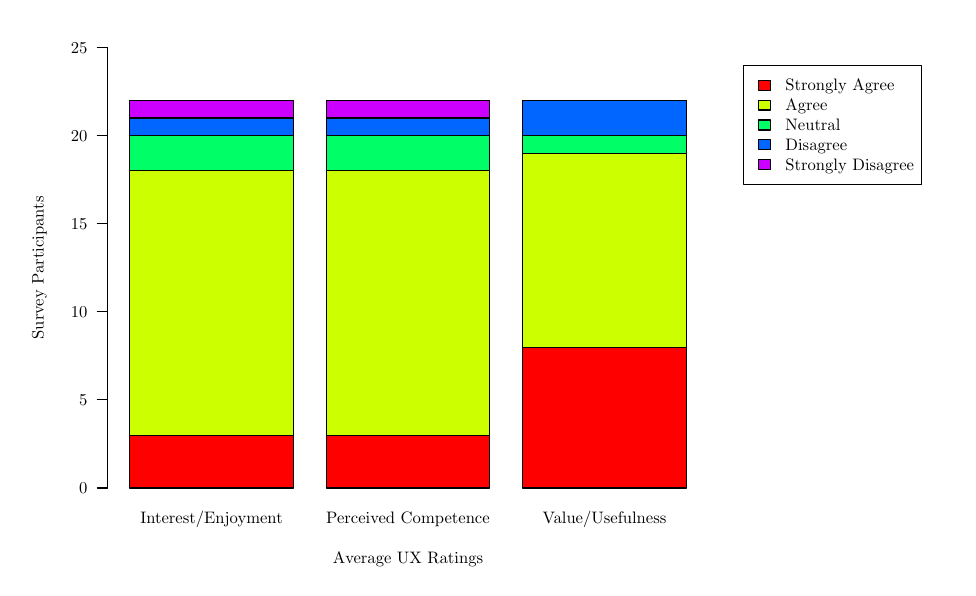
\begin{tikzpicture}[x=1pt,y=1pt]
\definecolor[named]{fillColor}{rgb}{1.00,1.00,1.00}
\path[use as bounding box,fill=fillColor,fill opacity=0.00] (0,0) rectangle (332.44,195.13);
\begin{scope}
\path[clip] (  0.00,  0.00) rectangle (332.44,195.13);
\definecolor[named]{drawColor}{rgb}{0.00,0.00,0.00}
\definecolor[named]{fillColor}{rgb}{1.00,0.00,0.00}

\path[draw=drawColor,line width= 0.4pt,line join=round,line cap=round,fill=fillColor] ( 36.85, 28.80) rectangle ( 96.01, 47.90);
\definecolor[named]{fillColor}{rgb}{0.80,1.00,0.00}

\path[draw=drawColor,line width= 0.4pt,line join=round,line cap=round,fill=fillColor] ( 36.85, 47.90) rectangle ( 96.01,143.37);
\definecolor[named]{fillColor}{rgb}{0.00,1.00,0.40}

\path[draw=drawColor,line width= 0.4pt,line join=round,line cap=round,fill=fillColor] ( 36.85,143.37) rectangle ( 96.01,156.10);
\definecolor[named]{fillColor}{rgb}{0.00,0.40,1.00}

\path[draw=drawColor,line width= 0.4pt,line join=round,line cap=round,fill=fillColor] ( 36.85,156.10) rectangle ( 96.01,162.47);
\definecolor[named]{fillColor}{rgb}{0.80,0.00,1.00}

\path[draw=drawColor,line width= 0.4pt,line join=round,line cap=round,fill=fillColor] ( 36.85,162.47) rectangle ( 96.01,168.83);
\definecolor[named]{fillColor}{rgb}{1.00,0.00,0.00}

\path[draw=drawColor,line width= 0.4pt,line join=round,line cap=round,fill=fillColor] (107.84, 28.80) rectangle (167.00, 47.90);
\definecolor[named]{fillColor}{rgb}{0.80,1.00,0.00}

\path[draw=drawColor,line width= 0.4pt,line join=round,line cap=round,fill=fillColor] (107.84, 47.90) rectangle (167.00,143.37);
\definecolor[named]{fillColor}{rgb}{0.00,1.00,0.40}

\path[draw=drawColor,line width= 0.4pt,line join=round,line cap=round,fill=fillColor] (107.84,143.37) rectangle (167.00,156.10);
\definecolor[named]{fillColor}{rgb}{0.00,0.40,1.00}

\path[draw=drawColor,line width= 0.4pt,line join=round,line cap=round,fill=fillColor] (107.84,156.10) rectangle (167.00,162.47);
\definecolor[named]{fillColor}{rgb}{0.80,0.00,1.00}

\path[draw=drawColor,line width= 0.4pt,line join=round,line cap=round,fill=fillColor] (107.84,162.47) rectangle (167.00,168.83);
\definecolor[named]{fillColor}{rgb}{1.00,0.00,0.00}

\path[draw=drawColor,line width= 0.4pt,line join=round,line cap=round,fill=fillColor] (178.83, 28.80) rectangle (238.00, 79.72);
\definecolor[named]{fillColor}{rgb}{0.80,1.00,0.00}

\path[draw=drawColor,line width= 0.4pt,line join=round,line cap=round,fill=fillColor] (178.83, 79.72) rectangle (238.00,149.74);
\definecolor[named]{fillColor}{rgb}{0.00,1.00,0.40}

\path[draw=drawColor,line width= 0.4pt,line join=round,line cap=round,fill=fillColor] (178.83,149.74) rectangle (238.00,156.10);
\definecolor[named]{fillColor}{rgb}{0.00,0.40,1.00}

\path[draw=drawColor,line width= 0.4pt,line join=round,line cap=round,fill=fillColor] (178.83,156.10) rectangle (238.00,168.83);
\definecolor[named]{fillColor}{rgb}{0.80,0.00,1.00}

\path[draw=drawColor,line width= 0.4pt,line join=round,line cap=round,fill=fillColor] (178.83,168.83) rectangle (238.00,168.83);
\end{scope}
\begin{scope}
\path[clip] (  0.00,  0.00) rectangle (332.44,195.13);
\definecolor[named]{drawColor}{rgb}{0.00,0.00,0.00}

\node[text=drawColor,anchor=base,inner sep=0pt, outer sep=0pt, scale=  0.60] at ( 66.43, 15.84) {Interest/Enjoyment};

\node[text=drawColor,anchor=base,inner sep=0pt, outer sep=0pt, scale=  0.60] at (137.42, 15.84) {Perceived Competence};

\node[text=drawColor,anchor=base,inner sep=0pt, outer sep=0pt, scale=  0.60] at (208.42, 15.84) {Value/Usefulness};
\end{scope}
\begin{scope}
\path[clip] (  0.00,  0.00) rectangle (332.44,195.13);
\definecolor[named]{drawColor}{rgb}{0.00,0.00,0.00}

\node[text=drawColor,anchor=base,inner sep=0pt, outer sep=0pt, scale=  0.60] at (137.42,  1.44) {Average UX Ratings};

\node[text=drawColor,rotate= 90.00,anchor=base,inner sep=0pt, outer sep=0pt, scale=  0.60] at (  5.76,108.36) {Survey Participants};
\end{scope}
\begin{scope}
\path[clip] (  0.00,  0.00) rectangle (332.44,195.13);
\definecolor[named]{drawColor}{rgb}{0.00,0.00,0.00}

\path[draw=drawColor,line width= 0.4pt,line join=round,line cap=round] ( 28.80, 28.80) -- ( 28.80,187.93);

\path[draw=drawColor,line width= 0.4pt,line join=round,line cap=round] ( 28.80, 28.80) -- ( 25.20, 28.80);

\path[draw=drawColor,line width= 0.4pt,line join=round,line cap=round] ( 28.80, 60.63) -- ( 25.20, 60.63);

\path[draw=drawColor,line width= 0.4pt,line join=round,line cap=round] ( 28.80, 92.45) -- ( 25.20, 92.45);

\path[draw=drawColor,line width= 0.4pt,line join=round,line cap=round] ( 28.80,124.28) -- ( 25.20,124.28);

\path[draw=drawColor,line width= 0.4pt,line join=round,line cap=round] ( 28.80,156.10) -- ( 25.20,156.10);

\path[draw=drawColor,line width= 0.4pt,line join=round,line cap=round] ( 28.80,187.93) -- ( 25.20,187.93);

\node[text=drawColor,anchor=base east,inner sep=0pt, outer sep=0pt, scale=  0.60] at ( 21.60, 26.73) {0};

\node[text=drawColor,anchor=base east,inner sep=0pt, outer sep=0pt, scale=  0.60] at ( 21.60, 58.56) {5};

\node[text=drawColor,anchor=base east,inner sep=0pt, outer sep=0pt, scale=  0.60] at ( 21.60, 90.39) {10};

\node[text=drawColor,anchor=base east,inner sep=0pt, outer sep=0pt, scale=  0.60] at ( 21.60,122.21) {15};

\node[text=drawColor,anchor=base east,inner sep=0pt, outer sep=0pt, scale=  0.60] at ( 21.60,154.04) {20};

\node[text=drawColor,anchor=base east,inner sep=0pt, outer sep=0pt, scale=  0.60] at ( 21.60,185.86) {25};
\end{scope}
\begin{scope}
\path[clip] (  0.00,  0.00) rectangle (332.44,195.13);
\definecolor[named]{drawColor}{rgb}{0.00,0.00,0.00}

\path[draw=drawColor,line width= 0.4pt,line join=round,line cap=round] (258.70,181.56) rectangle (323.00,138.36);
\definecolor[named]{fillColor}{rgb}{1.00,0.00,0.00}

\path[draw=drawColor,line width= 0.4pt,line join=round,line cap=round,fill=fillColor] (264.10,176.16) rectangle (268.42,172.56);
\definecolor[named]{fillColor}{rgb}{0.80,1.00,0.00}

\path[draw=drawColor,line width= 0.4pt,line join=round,line cap=round,fill=fillColor] (264.10,168.96) rectangle (268.42,165.36);
\definecolor[named]{fillColor}{rgb}{0.00,1.00,0.40}

\path[draw=drawColor,line width= 0.4pt,line join=round,line cap=round,fill=fillColor] (264.10,161.76) rectangle (268.42,158.16);
\definecolor[named]{fillColor}{rgb}{0.00,0.40,1.00}

\path[draw=drawColor,line width= 0.4pt,line join=round,line cap=round,fill=fillColor] (264.10,154.56) rectangle (268.42,150.96);
\definecolor[named]{fillColor}{rgb}{0.80,0.00,1.00}

\path[draw=drawColor,line width= 0.4pt,line join=round,line cap=round,fill=fillColor] (264.10,147.36) rectangle (268.42,143.76);

\node[text=drawColor,anchor=base west,inner sep=0pt, outer sep=0pt, scale=  0.60] at (273.82,172.30) {Strongly Agree};

\node[text=drawColor,anchor=base west,inner sep=0pt, outer sep=0pt, scale=  0.60] at (273.82,165.10) {Agree};

\node[text=drawColor,anchor=base west,inner sep=0pt, outer sep=0pt, scale=  0.60] at (273.82,157.90) {Neutral};

\node[text=drawColor,anchor=base west,inner sep=0pt, outer sep=0pt, scale=  0.60] at (273.82,150.70) {Disagree};

\node[text=drawColor,anchor=base west,inner sep=0pt, outer sep=0pt, scale=  0.60] at (273.82,143.50) {Strongly Disagree};
\end{scope}
\end{tikzpicture}

% }
\end{figure}
\end{frame}

\begin{frame}
\begin{figure}
 \centering
% \framebox[\texwidth]{
 % Created by tikzDevice version 0.6.2-92-0ad2792 on 2012-09-16 01:19:01
% !TEX encoding = UTF-8 Unicode
\begin{tikzpicture}[x=1pt,y=1pt]
\definecolor[named]{fillColor}{rgb}{1.00,1.00,1.00}
\path[use as bounding box,fill=fillColor,fill opacity=0.00] (0,0) rectangle (332.44,195.13);
\begin{scope}
\path[clip] (  0.00,  0.00) rectangle (332.44,195.13);
\definecolor[named]{drawColor}{rgb}{0.00,0.00,1.00}

\path[draw=drawColor,line width= 0.4pt,line join=round,line cap=round] ( 38.71, 50.90) --
	(100.67, 61.22) --
	(162.62, 73.00) --
	(224.58, 96.58) --
	(286.53,167.30);

\path[draw=drawColor,line width= 0.4pt,line join=round,line cap=round] ( 38.71, 50.90) circle (  1.35);

\path[draw=drawColor,line width= 0.4pt,line join=round,line cap=round] (100.67, 61.22) circle (  1.35);

\path[draw=drawColor,line width= 0.4pt,line join=round,line cap=round] (162.62, 73.00) circle (  1.35);

\path[draw=drawColor,line width= 0.4pt,line join=round,line cap=round] (224.58, 96.58) circle (  1.35);

\path[draw=drawColor,line width= 0.4pt,line join=round,line cap=round] (286.53,167.30) circle (  1.35);
\end{scope}
\begin{scope}
\path[clip] (  0.00,  0.00) rectangle (332.44,195.13);
\definecolor[named]{drawColor}{rgb}{0.00,0.00,0.00}

\path[draw=drawColor,line width= 0.4pt,line join=round,line cap=round] ( 38.71, 28.80) -- (286.53, 28.80);

\path[draw=drawColor,line width= 0.4pt,line join=round,line cap=round] ( 38.71, 28.80) -- ( 38.71, 25.20);

\path[draw=drawColor,line width= 0.4pt,line join=round,line cap=round] (100.67, 28.80) -- (100.67, 25.20);

\path[draw=drawColor,line width= 0.4pt,line join=round,line cap=round] (162.62, 28.80) -- (162.62, 25.20);

\path[draw=drawColor,line width= 0.4pt,line join=round,line cap=round] (224.58, 28.80) -- (224.58, 25.20);

\path[draw=drawColor,line width= 0.4pt,line join=round,line cap=round] (286.53, 28.80) -- (286.53, 25.20);

\node[text=drawColor,anchor=base,inner sep=0pt, outer sep=0pt, scale=  0.60] at ( 38.71, 15.84) {1,024};

\node[text=drawColor,anchor=base,inner sep=0pt, outer sep=0pt, scale=  0.60] at (100.67, 15.84) {2,048};

\node[text=drawColor,anchor=base,inner sep=0pt, outer sep=0pt, scale=  0.60] at (162.62, 15.84) {4,096};

\node[text=drawColor,anchor=base,inner sep=0pt, outer sep=0pt, scale=  0.60] at (224.58, 15.84) {8,192};

\node[text=drawColor,anchor=base,inner sep=0pt, outer sep=0pt, scale=  0.60] at (286.53, 15.84) {16,384};

\path[draw=drawColor,line width= 0.4pt,line join=round,line cap=round] ( 28.80, 34.69) -- ( 28.80,182.04);

\path[draw=drawColor,line width= 0.4pt,line join=round,line cap=round] ( 28.80, 34.69) -- ( 25.20, 34.69);

\path[draw=drawColor,line width= 0.4pt,line join=round,line cap=round] ( 28.80, 64.16) -- ( 25.20, 64.16);

\path[draw=drawColor,line width= 0.4pt,line join=round,line cap=round] ( 28.80, 93.63) -- ( 25.20, 93.63);

\path[draw=drawColor,line width= 0.4pt,line join=round,line cap=round] ( 28.80,123.10) -- ( 25.20,123.10);

\path[draw=drawColor,line width= 0.4pt,line join=round,line cap=round] ( 28.80,152.57) -- ( 25.20,152.57);

\path[draw=drawColor,line width= 0.4pt,line join=round,line cap=round] ( 28.80,182.04) -- ( 25.20,182.04);

\node[text=drawColor,anchor=base east,inner sep=0pt, outer sep=0pt, scale=  0.60] at ( 21.60, 32.63) {0};

\node[text=drawColor,anchor=base east,inner sep=0pt, outer sep=0pt, scale=  0.60] at ( 21.60, 62.10) {2};

\node[text=drawColor,anchor=base east,inner sep=0pt, outer sep=0pt, scale=  0.60] at ( 21.60, 91.56) {4};

\node[text=drawColor,anchor=base east,inner sep=0pt, outer sep=0pt, scale=  0.60] at ( 21.60,121.03) {6};

\node[text=drawColor,anchor=base east,inner sep=0pt, outer sep=0pt, scale=  0.60] at ( 21.60,150.50) {8};

\node[text=drawColor,anchor=base east,inner sep=0pt, outer sep=0pt, scale=  0.60] at ( 21.60,179.97) {10};
\end{scope}
\begin{scope}
\path[clip] (  0.00,  0.00) rectangle (332.44,195.13);
\definecolor[named]{drawColor}{rgb}{1.00,0.00,0.00}

\path[draw=drawColor,line width= 0.4pt,dash pattern=on 4pt off 4pt ,line join=round,line cap=round] ( 38.71, 45.01) --
	(100.67, 43.53) --
	(162.62, 43.53) --
	(224.58, 46.48) --
	(286.53, 47.95);

\path[draw=drawColor,line width= 0.4pt,line join=round,line cap=round] ( 37.52, 43.81) rectangle ( 39.91, 46.20);

\path[draw=drawColor,line width= 0.4pt,line join=round,line cap=round] ( 99.47, 42.34) rectangle (101.86, 44.73);

\path[draw=drawColor,line width= 0.4pt,line join=round,line cap=round] (161.42, 42.34) rectangle (163.82, 44.73);

\path[draw=drawColor,line width= 0.4pt,line join=round,line cap=round] (223.38, 45.28) rectangle (225.77, 47.68);

\path[draw=drawColor,line width= 0.4pt,line join=round,line cap=round] (285.33, 46.76) rectangle (287.73, 49.15);
\definecolor[named]{drawColor}{rgb}{0.00,0.00,0.00}

\node[text=drawColor,anchor=base,inner sep=0pt, outer sep=0pt, scale=  0.60] at (162.62,  1.44) {Files in Directory};

\node[text=drawColor,rotate= 90.00,anchor=base,inner sep=0pt, outer sep=0pt, scale=  0.60] at (  5.76,108.36) {Time (Seconds)};

\path[draw=drawColor,line width= 0.4pt,line join=round,line cap=round] ( 38.71,182.04) rectangle ( 90.14,160.44);
\definecolor[named]{drawColor}{rgb}{0.00,0.00,1.00}

\path[draw=drawColor,line width= 0.4pt,line join=round,line cap=round] ( 40.33,174.84) -- ( 51.13,174.84);
\definecolor[named]{drawColor}{rgb}{1.00,0.00,0.00}

\path[draw=drawColor,line width= 0.4pt,dash pattern=on 4pt off 4pt ,line join=round,line cap=round] ( 40.33,167.64) -- ( 51.13,167.64);
\definecolor[named]{drawColor}{rgb}{0.00,0.00,1.00}

\path[draw=drawColor,line width= 0.4pt,line join=round,line cap=round] ( 45.73,174.84) circle (  1.35);
\definecolor[named]{drawColor}{rgb}{1.00,0.00,0.00}

\path[draw=drawColor,line width= 0.4pt,line join=round,line cap=round] ( 44.54,166.44) rectangle ( 46.93,168.83);
\definecolor[named]{drawColor}{rgb}{0.00,0.00,0.00}

\node[text=drawColor,anchor=base west,inner sep=0pt, outer sep=0pt, scale=  0.60] at ( 56.53,172.77) {Initial Load};

\node[text=drawColor,anchor=base west,inner sep=0pt, outer sep=0pt, scale=  0.60] at ( 56.53,165.57) {Page Load};
\end{scope}
\end{tikzpicture}

% }
\end{figure}
\end{frame}
